\scanpage{35}
\uline{Quadriques}\quad Une base pour l'équivalence linéaire dans
$Q^{2n}$ est \unsure{formé|formée} de
\[
1,H,H^2\ldots H^{n-1},
\underbrace{S',S''}_{\text{codim }n},
HS'=HS'',\ldots H^nS'=H^nS''.
\]
\margin{On a $H^n=S'+S''$}
[$H$ est une section hyperplane dans l'immersion projective évidente;
$S'$ et $S''$ sont définis par des sous-espaces
\deleted{affines}\inserted{\uline{linéaires de \unsure{dim $n$}}}
dans $Q^{2n}$, appartenant aux deux familles algébriques distinctes
de tels sous-espaces.]

Une base de $Q^{2n+1}$ est formée de
\[
1,H,\ldots H^n,\frac{H^{n+1}}2,\ldots,\frac{H^{2n+1}}2.
\]
[ici $H$ est une section hyperplane, et ici les derniers
$\frac{H^{n+1}}2\ldots\frac{H^{2n+1}}2$ correspondent aux sous-variétés
linéaires contenues dans $Q^{2n+1}$]
\figure{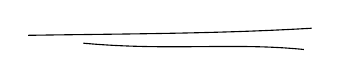
\begin{tikzpicture}
\draw (0,0) .. controls (1.3,.02) and (2.4,.02) .. (3.6,.09);
\draw (.7,-.10) .. controls (1.8,-.20) and (2.6,-.09) .. (3.5,-.18);
\end{tikzpicture}}
\mspage{34}
